\subsection{Consistency of local Voronoi diagrams}
\label{sec:localVoronoi}

In this section, we prove that the local and global Voronoi diagrams are the same within a particular distance from LiDAR.
%
A part of the track boundaries may not be \emph{visible} due to two reasons: being out of LiDAR's range, or occluded by other track boundaries.


Let $R$ be the range of LiDAR, 
and $d$ be the minimum distance of the track boundaries to LiDAR.
%
If $d \leq R$ then at least one point on the track boundaries is visible to LiDAR, so the local Voronoi diagram can be defined.
%
For any visible point $v$ on the track boundaries we have $d \leq \lVert v \rVert \leq R$ where $ \lVert \cdot \rVert $ is the Euclidean norm in LiDAR's coordinates.
%
We have the following guarantees:

\begin{figure}
\centering
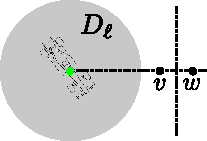
\includegraphics[width=4cm]{Figures/voronoi_occlusion.pdf}
\caption{If the Voronoi cell of a point in $D_\ell$ is identified by a track boundary $w$, then no track boundary $v$ occludes $w$. The green dot is LiDAR.}
\label{fig:voronoi-global-to-local}
\end{figure}

\begin{theorem}
Suppose that $d \leq R$.
%
Then the local and global Voronoi diagrams coincide on the disk $D_\ell$ of radius $\ell$ centered at LiDAR where
$$
\ell = \min \{ \frac{R-d}{2}, d \}.
$$
\label{thm:voronoi}
\end{theorem}

\begin{proof}
Let $p \in D_\ell$.
%
The global Voronoi cell of $p$ is identified with its closest track boundary points.
%
To prove that the local Voronoi cell of $p$ is the same as its global Voronoi cell, it is sufficient to show that all track boundary points closest to $p$ are visible.


Let $w$ be a track boundary closest to $p$.
%
We need to show that $w$ is visible.
%
By definition of $d$, there is a track boundary point $u$ with $\lVert u \rVert = d$.
%
By choice of $w$, we have
$$
\lVert p - w \rVert 
\leq \lVert p - u \rVert 
\leq \lVert p \rVert + \lVert u \rVert \leq \ell + d
$$
%
By definition of $\ell$, we have $\ell \leq \frac{R-d}{2}$, so
$$
\lVert w \rVert = \lVert w - p + p \rVert \leq \lVert w-p \rVert + \lVert p \rVert \leq 2\ell+d \leq R.
$$
%
This proves that $w$ is in range of LiDAR.
%
It remains to show that $w$ is not occluded.

Suppose, for the sake of contradiction, that $w$ is occluded.
%
That is,
there is a track boundary on the line segment between LiDAR and $w$.
%
Clearly, such points are in range since they are closer than $w$.
%
Choose $v$ to be such an occluding point that is the closest to LiDAR, so that $v$ is visible.
%
We must have $d \leq \lVert v \rVert $, by the definition of $d$.
%
Therefore, $\ell \leq d \leq \lVert v \rVert $.
%
Hence, all points in $D_\ell$ are closer to $v$ than to $w$, as shown in Fig~\ref{fig:voronoi-global-to-local}, since $D_\ell$ is on the left of the perpendicular bisector of the segment $vw$. 
%
In particular, $p$ is closer to $v$ than to $w$, which contradicts the choice of $w$.
%
Therefore, no such $v$ exists and $w$ is not occluded.
\end{proof}

Note that $D_\ell$ may not necessarily contain Voronoi \emph{edges} i.e. points that are equidistant from two or more different track boundary points.
%
Since our planner chooses a path on the Voronoi edges, we need to make sure that the set of Voronoi edges in $D_\ell$ is nonempty.
%
The following theorem gives sufficient lower bounds on LiDAR's range and distance to track boundaries.
%
Let $M$ be the maximum \emph{width} of the track.
%
That is, the distance between a global Voronoi edge and its closest track boundary is at most $\frac{M}{2}$.

\begin{theorem}
If $d \geq \frac{M}{4}$ and $R \geq \frac{3M}{2}$ then $D_\ell$ contains at least one point on the Voronoi edges.
\end{theorem}

\begin{proof}
First note that $d \leq \frac{M}{2}$ since LiDAR is \emph{on} the track i.e. between the left and right boundaries of the track.
%
Therefore, $R \geq \frac{3M}{2} \geq 3d$.
%
In particular, $R \geq d$, the local Voronoi diagram is defined and the previous theorem applies.
%
Furthermore,
$R-d \geq 2d$ so $\frac{R-d}{2} \geq d$.
%
Thus $\ell = \min \{ \frac{R-d}{2}, d \} = d$.
%
On the other hand, $d \geq \frac{M}{4}$ implies that $\frac{M}{2} \leq 2d = d + d$.
%
Hence $\frac{M}{2} \leq d + \ell $ so $\frac{M}{2} - d \leq \ell $.
%
However, if $p$ is a point closest to LiDAR and on the global Voronoi edges, we must have $\lVert p \rVert \leq \frac{M}{2} - d$.
%
Thus $p \in D_\ell$, so $p$ must be on a local Voronoi edge by the previous theorem.
\end{proof}

The condition $d \geq \frac{M}{4} = \frac{1}{2} \cdot \frac{M}{2}$ implies that LiDAR is at most half-way from global Voronoi edges to track boundaries.
%
This gives a convenient way to check whether global and local Voronoi diagrams are consistent, given a trajectory of the car and the map.